% !TeX program = pdflatex
% AntiFLipper (v11) -- every result table, figure and in-text number is generated by
% make_results.py from the experiment outputs. Run it before compiling.
\documentclass[conference]{IEEEtran}

\usepackage{amsmath,amssymb,amsfonts}
\usepackage{graphicx}
\usepackage{booktabs}
\usepackage{pifont}
\usepackage{url}
\usepackage{tikz}
\usetikzlibrary{arrows.meta,positioning,fit,backgrounds,calc,shapes.geometric,shapes.symbols,shadows}
\usepackage[ruled,vlined,linesnumbered]{algorithm2e}
\usepackage{cite}

\newtheorem{proposition}{Proposition}
% generated by make_results.py -- do not edit
\newcommand{\headAcc}{72.0}
\newcommand{\headAccRaw}{71.0}
\newcommand{\headAccFLTrust}{69.2}
\newcommand{\headAccLFighter}{59.0}
\newcommand{\headAccFLAME}{56.9}
\newcommand{\headAccFedAvg}{44.2}
\newcommand{\headAccKrum}{60.8}
\newcommand{\headAccKrumStd}{15.8}
\newcommand{\headFPRFLTrust}{0.44}
\newcommand{\headFPRRaw}{0.08}
\newcommand{\headFPRcc}{0.25}
\newcommand{\headFPRcconly}{0.00}
\newcommand{\headRecallLFighter}{0.46}
\newcommand{\headRecallFLAME}{0.42}
\newcommand{\headASR}{3.2}
\newcommand{\headASRFedAvg}{32.8}
\newcommand{\headDet}{15}
\newcommand{\defMs}{30}
\newcommand{\defMsFedAvg}{34}
\newcommand{\defMsFLTrust}{352}
\newcommand{\rootMsFLTrust}{115}
\newcommand{\defMsFLAME}{1058}
\newcommand{\defMsKrum}{875}
\newcommand{\defMsLFighter}{42}
\newcommand{\evalOverhead}{6.8}
\newcommand{\cleanHonRaw}{18.3}
\newcommand{\cleanHon}{0.0}
\newcommand{\cleanHonBudget}{8.0}
\newcommand{\cleanHonCC}{17.0}
\newcommand{\cleanHonZthree}{17.7}
\newcommand{\cleanAccRaw}{16.3}
\newcommand{\cleanAcc}{54.3}
\newcommand{\cleanAccCROnly}{60.2}
\newcommand{\cleanAccBudget}{16.8}
\newcommand{\cleanAccMid}{66.5}
\newcommand{\cleanAccMidRaw}{40.7}
\newcommand{\cleanHonMidRaw}{16.0}
\newcommand{\skewAcc}{49.1}
\newcommand{\skewAccStd}{11.9}
\newcommand{\skewAccFedAvg}{43.8}
\newcommand{\skewAccFedAvgStd}{9.1}
\newcommand{\skewAccLFighter}{41.6}
\newcommand{\skewAccFLTrust}{39.3}
\newcommand{\skewAccRaw}{13.0}
\newcommand{\skewFPRRaw}{0.94}
\newcommand{\skewRecall}{0.96}
\newcommand{\skewRecallLFighter}{0.21}
\newcommand{\skewRecallFLTrust}{0.58}
\newcommand{\skewDet}{70}
\newcommand{\fakeRecallRaw}{0.67}
\newcommand{\fakeRecallCROnly}{0.62}
\newcommand{\fakeRecall}{1.00}
\newcommand{\fakeAcc}{72.0}
\newcommand{\ratioAccLow}{74.1}
\newcommand{\ratioAccFedAvgLow}{74.3}
\newcommand{\ratioAccThirty}{72.4}
\newcommand{\ratioAccFedAvgThirty}{61.0}
\newcommand{\ratioAccLFighterThirty}{64.9}
\newcommand{\ratioAccFLTrustThirty}{70.8}
\newcommand{\bnsafeHead}{57.8}
\newcommand{\mnistAcc}{98.7}
\newcommand{\iidAcc}{73.3}
\newcommand{\skewFull}{2/3}
\newcommand{\skewDetHits}{70}
\newcommand{\skewMissed}{1}
\newcommand{\fltrustNanRuns}{3}
\newcommand{\fltrustNanRounds}{6}
\newcommand{\bnsafeFPR}{0.33}
\newcommand{\cleanFinal}{46.1}
\newcommand{\cleanFinalMin}{10.3}
\newcommand{\cleanAccStd}{9.8}
\newcommand{\cleanAccCROnlyStd}{7.5}
\newcommand{\ccOverrideShare}{0.6}
\newcommand{\ratioFPRmax}{0.14}
\newcommand{\matchedOurs}{173}
\newcommand{\matchedFedAvg}{183}
\newcommand{\matchedFLTrust}{1269}
\newcommand{\matchedKrum}{4109}
\newcommand{\matchedFLAME}{3465}
\newcommand{\matchedLFighter}{214}
\newcommand{\matchedRaw}{176}
\newcommand{\nRuns}{396}
\newcommand{\ccHeadAcc}{72.2}
\newcommand{\ccHeadFPR}{0.00}
\newcommand{\ccSkewAcc}{44.6}
\newcommand{\ccSkewRecall}{0.04}
\newcommand{\ccCleanAcc}{55.2}
\newcommand{\fsFound}{1}
\newcommand{\fsTotal}{24}
\newcommand{\fedWCleanAcc}{59.7}
\newcommand{\fedWCleanStd}{10.5}
\newcommand{\fedWCleanFinal}{62.2}
\newcommand{\fedWSkewAcc}{44.8}
\newcommand{\fedWSkewStd}{9.2}
\newcommand{\fedWSkewASR}{21.4}
\newcommand{\pfAccFedAvgHalf}{71.9}
\newcommand{\pfAccFedAvgQuarter}{73.6}
\newcommand{\fedCleanAcc}{57.6}
\newcommand{\fedCleanStd}{9.4}
\newcommand{\fedCleanFinal}{51.9}
\newcommand{\fedCleanMid}{65.0}
\newcommand{\fedCleanHigh}{75.1}
\newcommand{\pfAccHalf}{71.3}
\newcommand{\pfAccQuarter}{72.1}
\newcommand{\pfDetHalf}{24}
\newcommand{\pfDetQuarter}{39}
\newcommand{\fakeDet}{13}
\newcommand{\fsAcc}{43.1}
\newcommand{\fsRecall}{0.04}
\newcommand{\fsRecallCR}{0.00}
\newcommand{\sizeLowMin}{143}
\newcommand{\sizeLowMax}{10{,}704}
\newcommand{\sizeHighMin}{1{,}244}
\newcommand{\sizeHighMax}{4{,}835}
\newcommand{\aucHighMin}{0.73}
\newcommand{\aucHighMax}{0.91}
\newcommand{\aucLowMin}{0.56}
\newcommand{\aucLowMax}{0.65}
\newcommand{\trajSeed}{19}
\newcommand{\fsAccFedAvg}{43.8}
\newcommand{\cleanWinsFedW}{0}
\newcommand{\skewWinsFedW}{2}
\newcommand{\skewWinsFed}{3}
\newcommand{\skewASR}{7.5}
\newcommand{\skewASRFedAvg}{18.7}
\newcommand{\skewASRBest}{3}
\newcommand{\pfASRHalf}{3.2}
\newcommand{\pfASRQuarter}{3.2}
\newcommand{\pfASRFedAvgHalf}{5.0}
\newcommand{\pfASRFedAvgQuarter}{3.7}
\newcommand{\fakeAucResHighMin}{0.70}
\newcommand{\fakeAucResHighMax}{0.73}
\newcommand{\fakeAucRawLowMin}{0.64}
\newcommand{\fakeAucRawLowMax}{0.73}
\newcommand{\fakeAucResLowMin}{0.46}
\newcommand{\fakeAucResLowMax}{0.58}
\newcommand{\sensAccMin}{98.4}
\newcommand{\sensAccMax}{98.8}
\newcommand{\sensFPRmax}{0.09}
\newcommand{\sensRecallMin}{1.00}


\begin{document}

\title{\fontsize{21}{25}\selectfont AntiFLipper: A Secure and Efficient Defense Against\\ Label-Flipping Attacks in Federated Learning}

\author{\IEEEauthorblockN{Aashnan Rahman$^{1}$, Abid Hasan$^{2}$, Sherajul Arifin$^{3}$, Faisal Haque Bappy$^{4}$, Tahrim Hossain$^{5}$,\\ Tariqul Islam$^{6}$, Abu Raihan Mostofa Kamal$^{7}$, and Md. Azam Hossain$^{8}$}
\IEEEauthorblockA{
$^{1, 2, 7, 8}$ Islamic University of Technology, Bangladesh.\\
$^{3}$ United International University, Bangladesh.\\
$^{4, 5, 6}$ University of Maryland, Baltimore County, United States.}
}

\maketitle

\begin{abstract}
Federated learning (FL) trains a shared model without collecting client data, which leaves it open to label flipping, an attack in which malicious clients train on deliberately mislabelled data. A cheap defense that needs no clean data at the server is accuracy feedback, in which each client reports how well the global model fits its own labels and the server distrusts clients that report poorly. This defense breaks down when client data are heterogeneous, because honest clients that hold hard classes also report poorly, and because an attacker can simply report what an honest client would. We propose AntiFLipper, a lightweight defense that judges each report against the accuracy expected for the classes the client actually holds and pairs this class-conditional score with an inexpensive check of the client's last-layer update. It needs no server data, adds 84 bytes per client and round, and its server time is comparable to that of FedAvg. On CIFAR-10 with moderately skewed data and 40\% malicious clients, AntiFLipper reaches \headAcc\% accuracy, against at most \headAccFLTrust\% for six existing defenses, and excludes every attacker and no honest client, also when attackers fake reports or flip only some labels, and when only half of the clients take part. Under strongly skewed data it excludes no honest client, whereas raw feedback excluded \cleanHonRaw{} of 20, and with attackers it gives the lowest attack success rate of all methods in every run. Attackers that fake their reports under strong skew remain largely undetected.
\end{abstract}

\begin{IEEEkeywords}
Federated learning, label flipping, data poisoning, data heterogeneity, malicious client detection.
\end{IEEEkeywords}

% =============================================================================
\section{Introduction}
% =============================================================================
Federated learning (FL) trains a shared model across many clients, such as phones, sensors or hospitals, without collecting their data~\cite{fedavg-pmlr-v54-mcmahan17a,kairouz2021advances}. The server sees only model updates and cannot check how they were produced, which exposes FL to data poisoning~\cite{lyu2020threats}. In \emph{label flipping}, a malicious client relabels its data, for instance by swapping pairs of classes, and then trains as usual~\cite{biggio2011support,tolpegin2020data}. No change to the protocol or the training code is needed, yet enough such clients steer the global model towards systematic misclassification.

Detecting flippers is hard because honest clients differ as well. Each client holds its own mix of classes, and an unusual mix yields an unusual update. Defenses that inspect updates at the server, through robust statistics, distances or clustering~\cite{yin2018byzantine,NIPS2017_f4b9ec30,nguyen2022flame,jebreel2024lfighter}, are costly for large models and can mistake heterogeneous honest clients for attackers~\cite{li2023hscs,shen2024lfrppfl}. Defenses that score clients against clean data at the server~\cite{cao2020fltrust} need data that many deployments do not have.

A cheaper signal comes from the clients. If most clients are honest, the global model learns the true labels and fits a flipper's relabelled data poorly. Each client can evaluate the global model on its own data and report the result, and the server can lower the trust of clients that report poorly. This \emph{accuracy feedback} needs no server data and costs one forward pass per round~\cite{andreina2021baffle,jiang2023dataquality}. Used raw, however, it fails in two ways. First, an honest client that holds classes the model finds hard reports a low accuracy and is treated like an attacker. Under strong skew this effect cascades, because excluding such clients removes their classes from training and makes those classes harder still. Second, a report is only a claim, and a flipper can report what an honest client with the same data would report. Both problems grow with heterogeneity, exactly where update-based defenses struggle too.

We present \textbf{AntiFLipper}, which keeps the cost of accuracy feedback and addresses both failures. The server asks not whether a client's accuracy is low, but whether it is lower than \emph{expected for the classes that client holds}. A second check inspects what the client actually sent, so that a convincing report alone is not enough to stay trusted. The main contributions of this paper are as follows.
\begin{itemize}
\item \textbf{A label-mix-aware feedback defense.} AntiFLipper scores each report by a \emph{class-conditional residual}, the gap between the accuracy a client reports and the accuracy expected for its own label mix. It combines this score with a last-layer \emph{consistency check} of the update, keeps trust across rounds, and caps exclusions at the bound of the threat model.
\item \textbf{A lightweight, data-free design.} AntiFLipper needs no clean data at the server. Each client sends 84 bytes per round besides its update and adds \evalOverhead\% to its local training time, and the server work takes \matchedOurs\,ms per round, comparable to the \matchedFedAvg\,ms of FedAvg.
\item \textbf{Robustness to data heterogeneity.} Raw feedback excluded \cleanHonRaw{} of 20 honest clients under strong skew, whereas AntiFLipper excluded none at any level of skew. With 40\% attackers under strong skew, it gave the lowest attack success rate of all methods in every seed.
\item \textbf{Robustness to evasive attackers.} Under moderate skew, AntiFLipper excludes every attacker and no honest client also when attackers fake their reports or flip only part of their labels, and when only half of the clients take part in each round. It reaches \headAcc\% accuracy against at most \headAccFLTrust\% for six existing defenses on CIFAR-10.
\end{itemize}
We also report where AntiFLipper fails. Attackers that fake their reports under strong skew remain largely undetected, and Section~\ref{sec:analysis} traces this to a bias of the class-conditional estimate.

% =============================================================================
\section{Related Work}
\label{sec:related}
% =============================================================================
\textbf{Label flipping and data poisoning.} Label flipping was first studied as adversarial label noise in centralized learning, where flipping a small share of training labels already degrades support vector machines~\cite{biggio2011support}. Gradient-based poisoning extends the attack to deep networks~\cite{munoz2017towards}, and certified defenses bound its effect for convex learners~\cite{steinhardt2017certified}. In FL, flipping the labels of one class sharply reduces accuracy on that class even with a minority of attackers, and the damage grows with their share~\cite{tolpegin2020data}; its effect also depends strongly on how data are distributed~\cite{lavaur2024systematic}. Data poisoning is weak in production FL when attackers are very few~\cite{shejwalkar2022backdrawingboard}, so with up to 40\% malicious clients we model a stronger adversary. Crafted model updates~\cite{bhagoji2019analyzing,fang2020local,shejwalkar2021manipulating} and backdoors~\cite{bagdasaryan2020backdoor,wang2020attack,sun2019really} are different threats, since they alter the training procedure or target chosen inputs instead of running honest code on wrong labels.

\textbf{Robust aggregation.} Byzantine-robust rules bound the influence of any minority of updates. Median and Trimmed Mean~\cite{yin2018byzantine} aggregate each coordinate robustly, the geometric median~\cite{pillutla2022robust} aggregates whole updates, Multi-Krum~\cite{NIPS2017_f4b9ec30} keeps updates close to their neighbors, and Bulyan~\cite{mhamdi2018hidden} combines both but needs $N\ge4f+3$ clients for $f$ attackers. Centered clipping~\cite{karimireddy2021history} limits how far each update may move from the previous aggregate. These rules treat dissimilar updates as suspicious, yet under non-IID data honest updates are dissimilar too~\cite{zhao2018noniid,li2020federated}. Karimireddy et al.~\cite{karimireddy2022bucketing} show that robust rules can fail on heterogeneous data even against simple attacks, and they mix clients into random buckets before aggregating to restore robustness. The cost of these rules also grows with the size of the full model.

\textbf{Detection of malicious clients.} Detectors identify attackers and remove them instead of only bounding their influence. FoolsGold~\cite{fung2020limitations} down-weights clients with similar histories, FLAME~\cite{nguyen2022flame} clusters, clips and adds noise, CRFL~\cite{xie2021crfl} certifies robustness to backdoors, and FLDetector~\cite{zhang2022fldetector} flags clients whose updates disagree with a prediction from their own history. AUROR~\cite{shen2016auror} clusters indicative features of the updates. Against label flipping, Tolpegin et al.~\cite{tolpegin2020data} cluster last-layer updates and LFighter~\cite{jebreel2024lfighter} clusters the gradients of the most-changed output neurons. Clustering separates heterogeneous honest clients as readily as attackers~\cite{li2023hscs,shen2024lfrppfl}. Zeno~\cite{xie2019zeno}, FLTrust~\cite{cao2020fltrust} and HSCS~\cite{li2023hscs} avoid this by scoring clients against clean data at the server, which may be unavailable or unrepresentative.

\textbf{Feedback, trust and label quality.} In BaFFLe~\cite{andreina2021baffle}, clients validate each global model locally and vote on accepting it. Other schemes estimate the quality of each client's labels~\cite{jiang2023dataquality,ovi2023confident}, derive trust from a guiding signal~\cite{li2025flgt}, align client distributions at two granularities~\cite{fedalign2026}, or add a detection pipeline~\cite{abroshan2025aitoprotect}, and LFR-PPFL~\cite{shen2024lfrppfl} protects such statistics cryptographically. A separate line of work corrects benign label noise~\cite{song2023noisylabels}, also across federated clients~\cite{xu2022fedcorr}. It assumes clients that are noisy but cooperative, and it repairs labels rather than excluding clients. Feedback-based defenses avoid server data, but they generally read a low score as evidence of poisoning, which confuses poisoning with an unusual label mix, and they rarely consider attackers that lie about their score. AntiFLipper belongs to this family. It judges each report against what the client's own label mix predicts and pairs it with one cheap statistic of the update, without clustering or distances between full models.

% =============================================================================
\section{System and Threat Model}
\label{sec:model}
% =============================================================================
\textbf{System.} A server coordinates $N$ clients over $T$ rounds. Client $j$ holds a dataset $D_j$ with labels in $\{1,\dots,K\}$ and label mix $\pi_{jk}=n_{jk}/|D_j|$, where $n_{jk}$ is its number of class-$k$ samples. In round $t$, a set $S_t$ of clients sampled from those not excluded (all of them unless stated otherwise) receives the global model $M_t$, trains it for $E$ local epochs and returns the model $m_{j,t}$, together with a report that contains the accuracy $a_j$ of $M_t$ on its local labels, its per-class correct counts $\mathbf{c}_j$ and its per-class sample counts $\mathbf{n}_j$. The server keeps a trust value $\tau_j$ per client, normalized to sum to one, and a set $\beta$ of excluded clients.

\textbf{Adversary.} The adversary controls a fraction $p\le 0.4$ of the clients; staying below one half keeps coordinate-wise medians informative. Malicious clients relabel their data with the fixed permutation $\pi$: $0{\leftrightarrow}1$, $2{\leftrightarrow}3$, \dots, $8{\leftrightarrow}9$, and run the honest training code. A \emph{full flip} relabels all of a client's samples in every round. A \emph{partial flip} relabels a given fraction, drawn afresh at random in each round. Attackers report in one of two ways:
\begin{itemize}
\item \emph{Honest reporting:} statistics of $M_t$ on the labels the client trains on.
\item \emph{Report faking (adaptive):} statistics of $M_t$ on the client's \emph{original} labels, as an honest client with the same data would report.
\end{itemize}
Crafted updates such as gradient scaling or backdoors~\cite{bagdasaryan2020backdoor,fang2020local} are the domain of Byzantine-robust aggregation, with which AntiFLipper can be combined.

% =============================================================================
\section{Methodology}
\label{sec:design}
% =============================================================================
AntiFLipper answers each of the two failure modes with its own signal. The class-conditional residual corrects each report for label mix, and the consistency check observes the update instead of the report. Trust, flags and a capped exclusion rule turn both signals into an aggregation decision. Fig.~\ref{fig:arch} shows one round, and Algorithm~\ref{alg:af} lists the server side.

\begin{figure}[t]
\centering
\resizebox{\columnwidth}{!}{% AntiFLipper overview (one round). Included by AntiFlipper_v10.tex.
% Needs: \usetikzlibrary{arrows.meta,positioning,fit,backgrounds,calc,shapes.geometric,shapes.symbols}
% Grid: client lanes at x = 1.0 / 2.5 / 4.0; module bars start at x = 0.45;
%       M2/M5 end at x = 5.9; M4 occupies x = 6.45..8.25; M6 spans 0.45..8.25.
\definecolor{repc}{RGB}{38,99,170}\definecolor{repf}{RGB}{226,236,250}
\definecolor{updc}{RGB}{204,110,20}\definecolor{updf}{RGB}{253,237,219}
\definecolor{okc}{RGB}{22,150,100}\definecolor{badc}{RGB}{214,48,49}
\definecolor{barf}{RGB}{222,222,222}
\begin{tikzpicture}[
  font=\sffamily\small, >={Stealth[length=5pt,width=4pt]}, line cap=round,
  bar/.style={rounded corners=5pt, fill=barf, minimum height=0.62cm, align=center, inner sep=2pt},
  tok/.style={circle, minimum size=0.62cm, inner sep=0pt, font=\sffamily\footnotesize\bfseries},
  dia/.style={diamond, aspect=1, minimum size=0.82cm, inner sep=0pt, rounded corners=3pt, font=\sffamily\footnotesize\bfseries},
  group/.style={draw=black!45, dotted, line width=0.7pt, rounded corners=6pt},
  lbl/.style={font=\sffamily\scriptsize, align=left, text=black!75, anchor=west},
  w/.style={line width=0.9pt},
]
% ---------------------------------------------------------------- lanes and fixed columns
\def\xa{1.0}\def\xb{2.5}\def\xc{4.0}
\def\xl{4.6}   % left edge of the side labels
\def\xm{7.35}  % centre of M4
\def\ybus{0.95}
% ---------------------------------------------------------------- server frame (label sits on the frame line)
\draw[dashed, line width=0.8pt, rounded corners=9pt, black!70] (0.15,1.3) rectangle (8.55,7.05);
\node[font=\sffamily\small\bfseries, fill=white, inner sep=3pt, anchor=west] at (0.4,7.05) {Server};
% ---------------------------------------------------------------- clients (device card with a local data store)
\foreach \x/\n/\name/\col in {\xa/a/Client 1/black, \xb/b/Client 2/black, \xc/c/Attacker/badc}{
  \node[draw=\col, line width=1.1pt, rounded corners=4pt, minimum width=1.32cm, minimum height=0.95cm, fill=white] (cl\n) at (\x,0) {};
  \begin{scope}[shift={(\x-0.36,0.04)}, \col, line width=0.7pt]
    \draw[fill=white] (-0.16,0.16) -- (-0.16,-0.14) arc[start angle=180, end angle=360, x radius=0.16, y radius=0.055] -- (0.16,0.16);
    \draw[fill=white] (0,0.16) ellipse[x radius=0.16, y radius=0.055];
    \draw[line width=0.5pt] (-0.16,0.01) arc[start angle=180, end angle=360, x radius=0.16, y radius=0.055];
  \end{scope}
  \node[font=\sffamily\scriptsize, text=\col] at (\x+0.2,0.06) {$m_j$};
  \node[font=\sffamily\tiny, text=\col] at (\x,-0.33) {\name};
}
\node[font=\sffamily\tiny, text=badc, align=center, anchor=west] at (\xc+0.72,0.0) {flips\\labels};
% ---------------------------------------------------------------- M1: received reports
\node[group, minimum width=3.9cm, minimum height=0.95cm] at (\xb,2.05) {};
\foreach \x/\n/\c in {\xa/a/repc, \xb/b/repc, \xc/c/badc}
  \node[tok, fill=repf, draw=\c, line width=1.1pt] (r\n) at (\x,2.05) {M1};
\node[lbl] at (\xl,2.05) {Per-class\\reports (84\,B)};
% ---------------------------------------------------------------- M2
\node[bar, minimum width=5.45cm] (m2) at (3.175,3.1) {\textbf{M2:} Class-conditional residual \ $r_j$};
% ---------------------------------------------------------------- M3: per-client trust
\node[group, minimum width=3.9cm, minimum height=1.15cm] at (\xb,4.15) {};
\node[dia, fill=okc, text=white] (ta) at (\xa,4.15) {M3};
\node[dia, fill=okc, text=white] (tb) at (\xb,4.15) {M3};
\node[dia, fill=white, draw=badc, line width=1.1pt, text=badc] (tc) at (\xc,4.15) {M3};
\node[lbl] at (\xl,4.15) {Trust\\update $\tau_j$};
% ---------------------------------------------------------------- M5, M6
\node[bar, minimum width=5.45cm] (m5) at (3.175,5.15) {\textbf{M5:} Flags \& capped exclusion};
\node[bar, minimum width=7.8cm]  (m6) at (4.35,6.2)  {\textbf{M6:} Trust-weighted aggregation \ $\sum_{j\notin\beta}\tau_j m_j$};
% ---------------------------------------------------------------- M4 (update path): box with three stacked parts
\node[rounded corners=5pt, fill=updf, draw=updc, line width=0.9pt, minimum width=1.8cm, minimum height=3.9cm] (m4) at (\xm,3.55) {};
\node[align=center, anchor=north, inner sep=0pt] at ($(m4.north)+(0,-0.18)$) {\textbf{M4:}\\Update\\consistency\\check};
\draw[updc!60, line width=0.5pt] ($(m4.center)+(-0.6,0.1)$) -- ($(m4.center)+(0.6,0.1)$);
\node[font=\footnotesize] at ($(m4.center)+(0,-0.5)$) {$\cos(\delta_j,\tilde\delta)$};
\node[font=\sffamily\scriptsize, align=center, text=black!75] at ($(m4.center)+(0,-1.3)$) {last layer\\vs.\ median};
% ---------------------------------------------------------------- update bus (orange), clients -> M4
\foreach \n in {a,b,c}
  \draw[w, updc] ($(cl\n.north)+(0.42,0)$) -- ($(cl\n.north)+(0.42,\ybus-0.475)$);
\draw[w, updc, ->] ($(\xa+0.42,\ybus)$) -- (\xm,\ybus) -- (m4.south);
\node[font=\sffamily\scriptsize, text=updc, anchor=north] at (6.3,\ybus-0.04) {updates $m_j$};
% ---------------------------------------------------------------- report arrows (blue), centred on each M1, bridging the bus
\foreach \n/\c in {a/repc, b/repc, c/badc}
  \draw[w, \c, ->, preaction={draw=white, line width=3.4pt, shorten <=2pt, shorten >=2pt}] (cl\n.north) -- (r\n.south);
% ---------------------------------------------------------------- vertical flow through the modules
\foreach \n/\c in {a/black, b/black, c/badc}{
  \draw[w, \c, ->] (r\n.north) -- (r\n.north |- m2.south);
  \draw[w, \c, ->] (t\n.south |- m2.north) -- (t\n.south);
  \draw[w, \c, ->] (t\n.north) -- (t\n.north |- m5.south);
}
\foreach \x in {\xa,\xb}
  \draw[w, ->] (\x,5.46) -- (\x,5.89);
\draw[w, badc, dashed] (\xc,5.46) -- (\xc,5.6);
\node[circle, fill=badc, text=white, inner sep=0.6pt, font=\sffamily\tiny\bfseries] at (\xc,5.69) {$\times$};
\node[font=\sffamily\scriptsize, text=badc, anchor=west] at (\xc+0.18,5.69) {excluded};
% ---------------------------------------------------------------- M4 outputs
\draw[w, updc, ->] (m4.west |- m5) -- node[above, font=\sffamily\scriptsize, text=updc] {flag} (m5.east);
\draw[w, updc, ->] (m4.north) -- (m4.north |- m6.south);
% ---------------------------------------------------------------- global model and broadcast
\node[cloud, cloud puffs=11, cloud puff arc=110, aspect=2.2, draw=black!75, line width=0.9pt, fill=white,
      minimum width=2.3cm, minimum height=0.95cm, font=\sffamily\footnotesize, align=center] (gm) at (4.35,7.95) {Global model\\$M_{t+1}$};
\draw[w, ->] (m6.north) -- (gm.south);
\draw[w, ->] (gm.west) -- (-0.45,7.95) -- (-0.45,-0.95) -- (\xc,-0.95) -- (clc.south);
\foreach \n in {a,b} \draw[w, ->] (cl\n.south |- 0,-0.95) -- (cl\n.south);
\node[font=\sffamily\scriptsize, rotate=90, anchor=south] at (-0.45,3.4) {broadcast to active clients};
\end{tikzpicture}
}
\caption{One round of AntiFLipper. Each client sends a short report (blue) and its model update (orange). The server scores reports against each client's label mix, checks updates against the median, and aggregates only trusted clients; an attacker (red) is excluded.}
\label{fig:arch}
\end{figure}

\textbf{M1: Client report.} Before training, client $j$ runs one forward pass of $M_t$ over $D_j$ and records its accuracy $a_j$ and, for every class $k$, the numbers $c_{jk}$ of correct predictions and $n_{jk}$ of samples. With 32-bit values the payload is $4+8K$ bytes, i.e., 84 bytes for $K{=}10$.

\textbf{M2: Class-conditional residual.} The server pools per-class accuracy over clients, weighted by trust, and compares each report with the accuracy expected for that client's label mix:
\begin{equation}
\hat A_k=\frac{\sum_i \tau_i c_{ik}}{\sum_i \tau_i n_{ik}},\qquad
r_j=a_j-\sum_k \pi_{jk}\hat A_k .
\label{eq:cr}
\end{equation}
Classes without trust-weighted samples, and classes the client does not hold, are skipped. An honest client with hard classes reports a low $a_j$ but also has a low expectation, so its residual stays near zero. A flipper fits its own labels poorly in every class it holds, so its residual is negative, provided that $\hat A_k$ is dominated by honest clients. Because $\hat A_k$ includes the scored client's own report, this condition can fail for classes held mostly by flippers (Section~\ref{sec:analysis}).

\textbf{M3: Trust update.} With $\bar r$ the mean residual, trust moves by the squared deviation and is renormalized over the active clients:
\begin{equation}
\tau_j \leftarrow \max\!\big(0,\ \tau_j + \operatorname{sgn}(r_j-\bar r)\,\eta\,(r_j-\bar r)^2\big).
\label{eq:trust}
\end{equation}
The quadratic form damps small fluctuations and reacts strongly to persistent gaps.

\textbf{M4: Update-consistency check.} Let $\delta_j$ be the change of the classification layer (weights and bias) of client $j$ and $\tilde\delta$ the coordinate-wise median of all $\delta_j$. The server computes $s_j=\cos(\delta_j,\tilde\delta)$ and the robust score $(s_j-\operatorname{med}(s))/(1.4826\,\mathrm{MAD}(s)+\epsilon)$, with $\epsilon{=}10^{-6}$ for the case that all similarities coincide. A client scoring below $-z$ is \emph{inconsistent}. Its residual is replaced by the round minimum before~(\ref{eq:trust}), and it is flagged in M5.

\textbf{M5: Flags and capped exclusion.} After $g$ warm-up rounds, a client is flagged when $n_t\tau_j<\rho$, i.e., its trust falls below a fixed share of the uniform weight over the $n_t$ active clients, or when M4 marks it inconsistent. A client with $c_{\max}$ flags is excluded. Exclusions are capped at $b=\lfloor0.4N\rfloor$, the bound of the threat model; when more clients qualify, those with the lowest trust go first.

\textbf{M6: Aggregation.} $M_{t+1}=\sum_{j\in S_t\setminus\beta}\tau_j\,m_{j,t}\big/\sum_{j\in S_t\setminus\beta}\tau_j$. Trust persists for clients that are not sampled, and the flag test uses all $n_t$ active clients, so a sampled subset does not make every client look under-trusted.

\setlength{\textfloatsep}{8pt}
\begin{algorithm}[t]
\caption{AntiFLipper: server side of round $t$}
\label{alg:af}
\small
\KwIn{models $m_{j,t}$, reports $(a_j,\mathbf{c}_j,\mathbf{n}_j)$ for $j\in S_t$; trust $\tau$; flag counts $c$}
$\hat A_k\leftarrow\sum_i\tau_ic_{ik}\,/\sum_i\tau_in_{ik}$ \ for every $k$ with $\sum_i\tau_in_{ik}>0$\;
\lForEach{$j\in S_t$}{$r_j\leftarrow a_j-\sum_k \pi_{jk}\hat A_k$ \ over the classes defined above, $\pi_j$ renormalized}
$\tilde\delta\leftarrow$ coordinate-wise median of last-layer updates $\{\delta_j\}$\;
$s_j\leftarrow\cos(\delta_j,\tilde\delta)$; \ $I\leftarrow\{j:\ (s_j-\operatorname{med}(s))/(1.4826\,\mathrm{MAD}(s)+\epsilon)<-z\}$\;
\lForEach{$j\in I$}{$r_j\leftarrow\min_i r_i$}
update $\tau$ with~(\ref{eq:trust}) and normalize over $j\notin\beta$\;
\If{$t\ge g$}{
 \ForEach{$j\in S_t$}{\lIf{$n_t\tau_j<\rho$ \textbf{\upshape or} $j\in I$}{$c_j\leftarrow c_j+1$}}
 $Q\leftarrow\{j\notin\beta:\ c_j\ge c_{\max}\}$ sorted by increasing $\tau_j$\;
 add the first $\max(0,\,b-|\beta|)$ clients of $Q$ to $\beta$; normalize $\tau$\;
}
\Return $M_{t+1}=\sum_{j\in S_t\setminus\beta}\tau_j m_{j,t}/\sum_{j\in S_t\setminus\beta}\tau_j$
\end{algorithm}

% =============================================================================
\section{Experimental Setup}
\label{sec:setup}
% =============================================================================
\textbf{Data and models.} CIFAR-10~\cite{CIFAR-krizhevsky2009learning} is trained with ResNet-18~\cite{resnet-he2016deep} (11.2\,M parameters) over 20 clients and 100 rounds, and MNIST~\cite{MNIST-lecun1998gradient} with a CNN of 21.8\,k parameters over 100 clients and 200 rounds; IID and non-IID splits use the same number of clients. Non-IID splits divide the samples of each class among the clients in proportions drawn from $\mathrm{Dir}(\alpha_D)$, with $\alpha_D{=}1$ (moderate skew) unless stated otherwise and $\alpha_D{=}0.1$ for strong skew. Client datasets are therefore unequal in size. On CIFAR-10 they range from \sizeHighMin{} to \sizeHighMax{} samples at $\alpha_D{=}1$ and from \sizeLowMin{} to \sizeLowMax{} at $\alpha_D{=}0.1$. Unless stated otherwise all clients take part in every round; they train for $E{=}3$ epochs with SGD (learning rate 0.01, momentum 0.9, weight decay $5\cdot10^{-4}$, batch size 32 for CIFAR-10 and 64 for MNIST).

\textbf{Attacks.} By default 40\% of the clients perform a full flip and report honestly. This is the largest share our threat model allows and the hardest case, where undefended training and several baselines break down (Fig.~\ref{fig:ratio}). We also evaluate partial flips of 50\% and 25\%, partial participation (a random half of the active clients in every round), report faking at $\alpha_D{=}1$ and $0.1$, shares of 10--30\%, and runs without attackers, in which every exclusion is a false positive.

\textbf{Baselines.} We compare with FedAvg, coordinate-wise Median, Multi-Krum ($f=\lfloor pN\rfloor$), FLAME, LFighter and FLTrust. FLTrust additionally receives a class-balanced root set of 100 clean samples; its reference implementation rescales all tensors including BatchNorm statistics, so we also report a variant that rescales only trainable parameters. Bulyan is not applicable, as $N{=}20$ and $f{=}8$ violate $N\ge4f+3$. FedAvg denotes equal client weights, as AntiFLipper's initial trust; under strong skew we also run the original sample-weighted FedAvg~\cite{fedavg-pmlr-v54-mcmahan17a}. Ablations replace the residual with the raw report $a_j$, remove the consistency check (CC) or the cap, or use CC alone with uniform trust. All methods share partitions and attacker sets.

\textbf{Parameters and metrics.} AntiFLipper uses $\eta{=}0.1$, $\rho{=}0.05$, $c_{\max}{=}6$, $g{=}2$, $z{=}3$ and $b{=}0.4N$. Results are means and standard deviations over three seeds, \nRuns{} training runs in total; the sensitivity study uses separate held-out seeds. Accuracy and attack success rate (ASR, the share of test predictions equal to $\pi(y)$) are averaged over the last 10 rounds, since single rounds fluctuate by several points under strong skew. Precision, recall and false-positive rate (FPR) refer to the clients excluded, or given zero weight by baselines, in the final round. Server time covers all checks, trust updates and aggregation; we measure it during training, excluding rounds that overlapped other workloads, and in a matched benchmark that gives every method the same 20 updates.

% =============================================================================
\section{Results}
\label{sec:results}
% =============================================================================
\begin{table*}[t]
\centering
\caption{Comparison with existing defenses under 40\% label-flipping clients (mean$\pm$std over three seeds).}
\label{tab:main}
\footnotesize
\setlength{\tabcolsep}{4.5pt}
\begin{tabular}{@{}l ccccc c cc@{}}
\toprule
& \multicolumn{5}{c}{\textbf{CIFAR-10, non-IID} ($\alpha_D{=}1$)} & \textbf{CIFAR-10} & \multicolumn{2}{c}{\textbf{MNIST}} \\
\cmidrule(lr){2-6}\cmidrule(lr){7-7}\cmidrule(lr){8-9}
\textbf{Method} & Acc.\,(\%)\,$\uparrow$ & ASR\,(\%)\,$\downarrow$ & Prec.\,$\uparrow$ & Rec.\,$\uparrow$ & FPR\,$\downarrow$ & IID Acc. & non-IID Acc. & IID Acc. \\
\midrule
FedAvg & 44.2{\scriptsize$\pm$0.5} & 32.8 & n/a & n/a & n/a & 42.1{\scriptsize$\pm$0.1} & 49.8{\scriptsize$\pm$0.3} & 49.6{\scriptsize$\pm$0.1} \\
Median & 57.9{\scriptsize$\pm$4.2} & 16.7 & n/a & n/a & n/a & 62.9{\scriptsize$\pm$1.4} & -- & -- \\
Multi-Krum & 60.8{\scriptsize$\pm$15.8} & 12.5 & 0.60 & 0.75 & 0.33 & 72.9{\scriptsize$\pm$0.3} & -- & -- \\
FLAME & 56.9{\scriptsize$\pm$7.7} & 17.7 & 0.49 & 0.42 & 0.17 & 71.1{\scriptsize$\pm$0.4} & -- & -- \\
LFighter & 59.0{\scriptsize$\pm$13.3} & 15.2 & 0.71 & 0.46 & 0.08 & 73.2{\scriptsize$\pm$0.3} & 98.5{\scriptsize$\pm$0.2} & \textbf{98.7}{\scriptsize$\pm$0.1} \\
FLTrust (reference)$^{\dagger}$ & 69.2{\scriptsize$\pm$1.1} & 5.2 & 0.60 & 0.92 & 0.44 & 63.1{\scriptsize$\pm$0.3} & 97.2{\scriptsize$\pm$0.1} & 97.5{\scriptsize$\pm$0.1} \\
FLTrust (BN-safe)$^{\dagger}$ & 57.8{\scriptsize$\pm$1.2} & 15.1 & 0.23 & 0.29 & 0.33 & 63.9{\scriptsize$\pm$2.3} & -- & -- \\
\midrule
\textbf{AntiFLipper} & \textbf{72.0}{\scriptsize$\pm$0.6} & \textbf{3.2} & \textbf{1.00} & \textbf{1.00} & \textbf{0.00} & \textbf{73.3}{\scriptsize$\pm$0.4} & \textbf{98.7}{\scriptsize$\pm$0.1} & \textbf{98.7}{\scriptsize$\pm$0.2} \\
\bottomrule
\end{tabular}
\\[2pt]\parbox{\linewidth}{\scriptsize $^{\dagger}$Uses a 100-sample clean root dataset at the server. Reference: rescales all tensors including BatchNorm statistics; BN-safe: trainable parameters only.}
\end{table*}

\begin{table*}[t]
\centering
\caption{Ablation on CIFAR-10: AntiFLipper with components removed (mean over three seeds).}
\label{tab:ablation}
\footnotesize
\setlength{\tabcolsep}{3.6pt}
\begin{tabular}{@{}l ccc cc ccc ccc cc@{}}
\toprule
& & & & \multicolumn{2}{c}{\textbf{40\% attack}} & \multicolumn{3}{c}{\textbf{40\% report faking}} & \multicolumn{3}{c}{\textbf{No attack}} & \multicolumn{2}{c}{\textbf{40\% attack}} \\
& & & & \multicolumn{2}{c}{$\alpha_D{=}1$} & \multicolumn{3}{c}{$\alpha_D{=}1$} & \multicolumn{3}{c}{$\alpha_D{=}0.1$} & \multicolumn{2}{c}{$\alpha_D{=}0.1$} \\
\cmidrule(lr){5-6}\cmidrule(lr){7-9}\cmidrule(lr){10-12}\cmidrule(lr){13-14}
\textbf{Variant} & CR & CC & Cap & Acc. & FPR & Acc. & Rec. & FPR & Acc.\,(last 10) & Acc.\,(final) & Excl.\,$\downarrow$ & Acc. & Rec. \\
\midrule
FedAvg & -- & -- & -- & 44.2 & n/a & 44.2 & n/a & n/a & 57.6{\scriptsize$\pm$9.4} & 51.9{\scriptsize$\pm$22.6} & n/a & 43.8 & n/a \\
FedAvg (sample-weighted) & -- & -- & -- & -- & n/a & -- & n/a & n/a & 59.7{\scriptsize$\pm$10.5} & 62.2{\scriptsize$\pm$7.2} & n/a & 44.8 & n/a \\
\midrule
Raw reports & \ding{55} & \ding{55} & \ding{55} & 71.0 & 0.08 & 72.4 & 0.67 & 0.08 & 16.3{\scriptsize$\pm$5.9} & 16.9{\scriptsize$\pm$5.7} & 18.3 & 13.0 & 0.88 \\
Raw reports + cap & \ding{55} & \ding{55} & \ding{51} & -- & -- & -- & -- & -- & 16.8{\scriptsize$\pm$6.4} & 16.7{\scriptsize$\pm$6.1} & 8.0 & 12.5 & 0.38 \\
Raw reports + CC & \ding{55} & \ding{51} & \ding{55} & 70.4 & 0.25 & 71.6 & 0.88 & 0.17 & 31.2{\scriptsize$\pm$15.2} & 31.4{\scriptsize$\pm$15.0} & 17.0 & 28.9 & \textbf{0.96} \\
CC only$^{\ddagger}$ & -- & \ding{51} & \ding{51} & \textbf{72.2} & \textbf{0.00} & 72.2 & \textbf{1.00} & \textbf{0.00} & 55.2{\scriptsize$\pm$7.8} & 52.0{\scriptsize$\pm$22.7} & 0.3 & 44.6 & 0.04 \\
CR + cap (no CC) & \ding{51} & \ding{55} & \ding{51} & 70.7 & \textbf{0.00} & \textbf{73.5} & 0.62 & \textbf{0.00} & \textbf{60.2}{\scriptsize$\pm$7.5} & \textbf{63.3}{\scriptsize$\pm$7.0} & 0.3 & \textbf{49.1} & \textbf{0.96} \\
\midrule
\textbf{AntiFLipper} & \ding{51} & \ding{51} & \ding{51} & 72.0 & \textbf{0.00} & 72.0 & \textbf{1.00} & \textbf{0.00} & 54.3{\scriptsize$\pm$9.8} & 46.1{\scriptsize$\pm$31.1} & \textbf{0.0} & \textbf{49.1} & \textbf{0.96} \\
\bottomrule
\end{tabular}
\\[2pt]\parbox{\linewidth}{\scriptsize Acc.: last-10-round mean unless marked. Excl.: honest clients excluded (of 20). FedAvg rows: no defense, for reference; the sample-weighted one weights clients by dataset size and was run only at $\alpha_D{=}0.1$. --: not run. CC uses $z{=}2.5$ in ``Raw reports + CC'' and $z{=}3$ elsewhere. $^{\ddagger}$Uniform trust; it ignores reports, so faking has no effect.}
\end{table*}


\subsection{Comparison with existing defenses}
On CIFAR-10 non-IID with 40\% attackers (Table~\ref{tab:main}), AntiFLipper reaches \headAcc\% accuracy, the highest of all methods, and lowers the ASR from \headASRFedAvg\% under FedAvg to \headASR\%. In every seed it excludes all attackers, on average by round \headDet, and no honest client. The strongest baseline, the reference FLTrust, reaches \headAccFLTrust\% but needs server data, flags \headFPRFLTrust{} of the honest clients and produced non-finite losses in \fltrustNanRounds{} rounds across \fltrustNanRuns{} of its 3 runs; its BatchNorm-safe variant avoids these failures but reaches only \bnsafeHead\%. LFighter and FLAME find \headRecallLFighter{} and \headRecallFLAME{} of the attackers, and their accuracy, like that of Multi-Krum ($\pm$\headAccKrumStd), varies strongly across seeds. On CIFAR-10 IID and on MNIST, where heterogeneity is mild or absent, the strong methods lie within about a point of one another. The differences that matter appear with skewed data, which the next subsections examine.

\subsection{Honest clients under strong skew}
\begin{figure}[t]
\centering
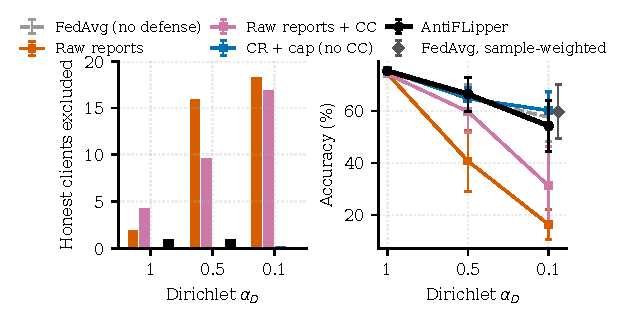
\includegraphics[width=\columnwidth]{fig/gen_heterogeneity.pdf}
\caption{Honest clients excluded (a) and test accuracy (b) on CIFAR-10 without attackers, as data become more skewed (smaller $\alpha_D$). Sample-weighted FedAvg was run at $\alpha_D{=}0.1$ only.}
\label{fig:het}
\end{figure}

\begin{figure}[t]
\centering
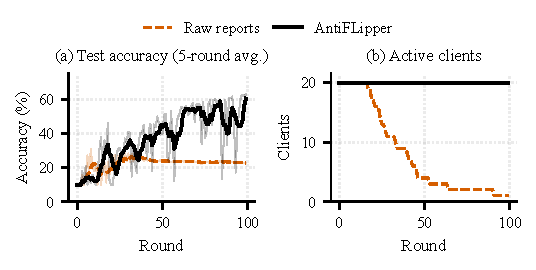
\includegraphics[width=\columnwidth]{fig/gen_trajectories.pdf}
\caption{Test accuracy (a) and active clients (b) per round in one run without attackers at $\alpha_D{=}0.1$ (seed \trajSeed, the middle of our three seeds by number, not by outcome). Raw reports exclude honest clients in a cascade, whereas AntiFLipper excludes none.}
\label{fig:traj}
\end{figure}

Without attackers every exclusion is a false positive (Fig.~\ref{fig:het}). Raw reports exclude \cleanHonMidRaw{} of 20 honest clients at $\alpha_D{=}0.5$ and \cleanHonRaw{} at $\alpha_D{=}0.1$, where accuracy collapses to \cleanAccRaw\%. Fig.~\ref{fig:traj} shows the resulting cascade, in which exclusions accumulate round after round (Section~\ref{sec:analysis} explains why). With the residual, exclusions stay near zero at every level of skew, and at $\alpha_D{=}0.5$ accuracy rises from \cleanAccMidRaw\% to \cleanAccMid\%.

The residual removes the penalty of raw feedback but does not make strongly skewed training more accurate than training without a defense. At $\alpha_D{=}0.1$, AntiFLipper averages \cleanAcc$\pm$\cleanAccStd\%, equal-weight FedAvg \fedCleanAcc$\pm$\fedCleanStd\% and sample-weighted FedAvg \fedWCleanAcc$\pm$\fedWCleanStd\%, which is ahead of AntiFLipper in each seed. As CC marked only \ccOverrideShare\% of client-rounds and no honest client was excluded, the gap stems from the trust weights, which shift the trajectory considerably at this skew. Without attackers, AntiFLipper thus costs a few points of accuracy under strong skew, in exchange for the protection measured next.

\subsection{Attackers under strong skew}
\begin{table}[t]
\centering
\caption{Strong skew with attackers (CIFAR-10, $\alpha_D{=}0.1$, 40\% full flips, honest reports).}
\label{tab:skew}
\footnotesize
\setlength{\tabcolsep}{3.6pt}
\begin{tabular}{@{}l ccccc@{}}
\toprule
\textbf{Method} & Acc.\,(\%)\,$\uparrow$ & ASR\,$\downarrow$ & Rec. & FPR & All found \\
\midrule
FedAvg & 43.8{\scriptsize$\pm$9.1} & 18.7 & n/a & n/a & n/a \\
FedAvg (weighted) & 44.8{\scriptsize$\pm$9.2} & 21.4 & n/a & n/a & n/a \\
LFighter & 41.6{\scriptsize$\pm$11.5} & 19.0 & 0.21 & 0.28 & n/a \\
FLTrust$^{\dagger}$ & 39.3{\scriptsize$\pm$6.5} & 16.0 & 0.58 & 0.53 & n/a \\
\midrule
Raw reports & 13.0{\scriptsize$\pm$2.6} & 15.8 & 0.88 & 0.94 & 0/3 \\
\textbf{AntiFLipper} & \textbf{49.1}{\scriptsize$\pm$11.9} & \textbf{7.5} & \textbf{0.96} & \textbf{0.00} & 2/3 (70) \\
\bottomrule
\end{tabular}
\\[2pt]\parbox{\linewidth}{\scriptsize FedAvg: equal client weights; weighted: by dataset size, as in~\cite{fedavg-pmlr-v54-mcmahan17a}. All found: seeds in which every attacker was excluded (mean round).}
\end{table}

Table~\ref{tab:skew} adds 40\% attackers at $\alpha_D{=}0.1$. AntiFLipper reaches \skewAcc\%, against \skewAccFedAvg\% for FedAvg, \fedWSkewAcc\% for sample-weighted FedAvg, \skewAccLFighter\% for LFighter and \skewAccFLTrust\% for FLTrust. Seed by seed it beats FedAvg in \skewWinsFed{} of 3 seeds and sample-weighted FedAvg in \skewWinsFedW, and its ASR (\skewASR\%, against \skewASRFedAvg\% and \fedWSkewASR\%) is the lowest of all methods in each of the \skewASRBest{} seeds; weighting by size raises the ASR, as large attackers gain influence. AntiFLipper finds \skewRecall{} of the attackers without excluding an honest client, whereas raw reports flag \skewFPRRaw{} of the honest clients. Detection is slower and not always complete. All attackers were excluded in \skewFull{} seeds, by round \skewDetHits{} on average, and in the third seed \skewMissed{} attacker remained. The probability that a random unmarked attacker has a lower residual than a random honest client (the AUC, averaged over the first ten rounds) is \aucHighMin--\aucHighMax{} per seed at $\alpha_D{=}1$ but only \aucLowMin--\aucLowMax{} at $\alpha_D{=}0.1$, consistent with the estimation bias of Section~\ref{sec:analysis}.

\subsection{Attackers that try to stay hidden}
\label{sec:hidden}
\begin{table*}[t]
\centering
\caption{Partial flips and partial participation (CIFAR-10 non-IID, $\alpha_D{=}1$, 40\% attackers, mean over three seeds).}
\label{tab:partial}
\footnotesize
\setlength{\tabcolsep}{3.4pt}
\begin{tabular}{@{}l cccc cccc cccc@{}}
\toprule
& \multicolumn{4}{c}{\textbf{Partial flip, 50\% of labels}} & \multicolumn{4}{c}{\textbf{Partial flip, 25\% of labels}} & \multicolumn{4}{c}{\textbf{Full flip, 50\% participation}} \\
\cmidrule(lr){2-5}\cmidrule(lr){6-9}\cmidrule(l){10-13}
\textbf{Method} & Acc.\,(\%) & ASR & Rec. & FPR & Acc.\,(\%) & ASR & Rec. & FPR & Acc.\,(\%) & ASR & Rec.$^{*}$ & FPR$^{*}$ \\
\midrule
FedAvg & \textbf{71.9} & 5.0 & n/a & n/a & \textbf{73.6} & 3.7 & n/a & n/a & 46.1{\scriptsize$\pm$3.0} & 30.6 & n/a & n/a \\
LFighter & 70.4 & 4.2 & 0.46 & 0.08 & 72.3 & 3.7 & 0.17 & 0.14 & 63.6{\scriptsize$\pm$6.5} & 10.0 & 0.84 & 0.13 \\
FLTrust (BN-safe)$^{\dagger}$ & 70.5 & 4.5 & 0.67 & 0.31 & 66.1 & 4.3 & 0.50 & 0.19 & 62.1{\scriptsize$\pm$2.6} & 11.1 & 0.50 & 0.15 \\
\midrule
\textbf{AntiFLipper} & 71.3 & \textbf{3.2} & \textbf{1.00} & \textbf{0.00} & 72.1 & \textbf{3.2} & \textbf{1.00} & \textbf{0.00} & \textbf{71.0}{\scriptsize$\pm$1.0} & \textbf{3.3} & \textbf{1.00} & \textbf{0.00} \\
\bottomrule
\end{tabular}
\\[2pt]\parbox{\linewidth}{\scriptsize Partial flip: share of each attacker's samples relabelled, a fresh random subset in every round; all clients take part. Participation: a random half of the active clients is sampled in every round. $^{\dagger}$BN-safe aggregation and a 100-sample clean root set. $^{*}$AntiFLipper: clients excluded in the final round. Baselines down-weight only the clients sampled in a round, so for them we report the share of sampled attackers (honest clients) given zero weight over the last 10 rounds.}
\end{table*}

\begin{table}[t]
\centering
\caption{Attackers that try to stay hidden (CIFAR-10, 40\% attackers).}
\label{tab:adaptive}
\footnotesize
\setlength{\tabcolsep}{2.4pt}
\begin{tabular}{@{}l c cc ccccc@{}}
\toprule
& & \multicolumn{2}{c}{\textbf{FedAvg}} & \multicolumn{5}{c}{\textbf{AntiFLipper}} \\
\cmidrule(lr){3-4}\cmidrule(l){5-9}
\textbf{Attack} & $\alpha_D$ & Acc. & ASR & Acc.\,(\%) & ASR & Rec. & FPR & Found \\
\midrule
Full flip & 1 & 44.2 & 32.8 & 72.0{\scriptsize$\pm$0.6} & 3.2 & 1.00 & 0.00 & 3/3 (15) \\
\midrule
Partial, 50\% & 1 & 71.9 & 5.0 & 71.3{\scriptsize$\pm$0.4} & 3.2 & 1.00 & 0.00 & 3/3 (24) \\
Partial, 25\% & 1 & 73.6 & 3.7 & 72.1{\scriptsize$\pm$0.5} & 3.2 & 1.00 & 0.00 & 3/3 (39) \\
\midrule
Faking & 1 & 44.2 & 32.8 & 72.0{\scriptsize$\pm$0.3} & 3.3 & 1.00 & 0.00 & 3/3 (13) \\
Faking & 0.1 & 43.8 & 18.7 & 43.1{\scriptsize$\pm$9.8} & 17.2 & 0.04 & 0.06 & 0/3 \\
\quad CR only$^{*}$ & 0.1 & -- & -- & 44.5{\scriptsize$\pm$7.4} & 17.2 & 0.00 & 0.00 & 0/3 \\
\quad CC only$^{\ddagger}$ & 0.1 & -- & -- & 44.6{\scriptsize$\pm$7.6} & 19.0 & 0.04 & 0.03 & 0/3 \\
\bottomrule
\end{tabular}
\\[2pt]\parbox{\linewidth}{\scriptsize Partial: share of each attacker's samples relabelled, a fresh random subset in every round. FedAvg ignores reports, so its faking rows repeat the honest-reporting runs. $^{*}$Residual and cap, no consistency check. $^{\ddagger}$Consistency check and cap with uniform trust; it ignores reports, so its row is the honest-reporting run. Found: seeds in which every attacker was excluded (mean round).}
\end{table}

\textbf{Partial flips.} An attacker that flips only part of its labels reports a higher accuracy and moves the model less. At both tested fractions AntiFLipper still excludes every attacker without false positives, by round \pfDetHalf{} at 50\% and \pfDetQuarter{} at 25\% (Table~\ref{tab:partial}). LFighter finds only \pfRecLFighterHalf{} and \pfRecLFighterQuarter{} of the attackers and the BN-safe FLTrust \pfRecFLTrustHalf{} and \pfRecFLTrustQuarter, both with false positives. These attacks are weak, however, and FedAvg still reaches \pfAccFedAvgHalf\% and \pfAccFedAvgQuarter\%, slightly above AntiFLipper (\pfAccHalf\% and \pfAccQuarter\%), which loses the correctly labelled part of the excluded clients' data. Partial flips thus show that detection survives a weaker signal, not that it improves accuracy.

\textbf{Report faking under moderate skew.} AntiFLipper detects every faker, by round \fakeDet{} on average, with no false positives. Raw reports find \fakeRecallRaw{} of them and the residual alone \fakeRecallCROnly. Report-only variants find some fakers because the model has trained on their flipped samples, a leakage discussed in Section~\ref{sec:analysis}. The residual of faked reports therefore still ranks attackers below honest clients (AUC \fakeAucResHighMin--\fakeAucResHighMax), but too weakly to exclude them all, and the consistency check catches the rest.

\textbf{Report faking under strong skew.} Here faking succeeds. AntiFLipper finds \fsRecall{} of the attackers (\fsFound{} of \fsTotal{} over three seeds), and its accuracy (\fsAcc\%) is no better than that of FedAvg (\fsAccFedAvg\%). The logs show why. The raw faked reports still rank attackers below honest clients (AUC \fakeAucRawLowMin--\fakeAucRawLowMax), but the residual reduces this to \fakeAucResLowMin--\fakeAucResLowMax. Under strong skew each class is concentrated on a few clients, so for classes held mostly by attackers, $\hat A_k$ consists largely of their own reports and absorbs their deficit, the bias of Section~\ref{sec:analysis}. The consistency check alone finds \ccSkewRecall{} of the attackers, because honest updates already differ widely. This is the main open case; a reference that leaves out the scored client, or a robust per-class estimate, are natural next steps.

\subsection{Partial participation}
\label{sec:participation}
In cross-device FL only part of the clients take part in a round. With a random half of the active clients sampled in every round (Table~\ref{tab:partial}, right), AntiFLipper reaches \ppAcc$\pm$\ppAccStd\%, close to its \headAcc\% with full participation, and again excludes every attacker without false positives in \ppFull{} seeds. Detection is slower (round \ppDet{} on average instead of \headDet), because each client collects flags only in the rounds in which it is sampled. LFighter reaches \ppAccLFighter$\pm$\ppAccLFighterStd\%, the BN-safe FLTrust \ppAccFLTrust\% and FedAvg \ppAccFedAvg\%, with ASRs of \ppASRLFighter\%, \ppASRFLTrust\% and \ppASRFedAvg\% against \ppASR\% for AntiFLipper. Baselines judge each round anew, whereas persistent trust lets AntiFLipper use evidence from every round in which a client took part.

\subsection{Ablation}
Table~\ref{tab:ablation} attributes these results to components. In the main setting all feedback variants perform similarly, and CC alone, with the same $z$ and cap, is as accurate as AntiFLipper (\ccHeadAcc\%). The harder settings separate them. Raw reports fail without attackers under strong skew and against report faking, and the cap alone only limits the damage (\cleanHonBudget{} honest clients excluded instead of \cleanHonRaw). The residual prevents these exclusions but misses fakers. CC alone catches every faker but finds only \ccSkewRecall{} of the attackers under strong skew. Each signal thus covers the failure of the other, and only the combination does well in all three settings. The combination is not best everywhere, since without attackers under strong skew the residual alone is more accurate.

\subsection{Share of malicious clients}
\begin{figure}[t]
\centering
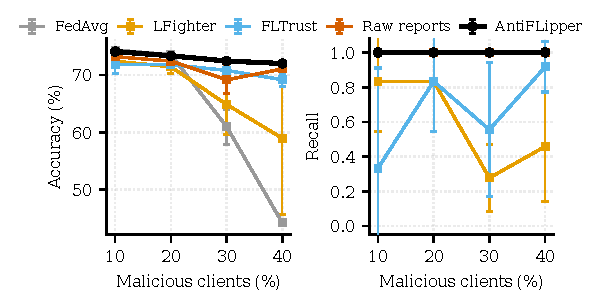
\includegraphics[width=\columnwidth]{fig/gen_ratio.pdf}
\caption{Test accuracy (a) and recall (b) on CIFAR-10 non-IID ($\alpha_D{=}1$) versus the share of malicious clients.}
\label{fig:ratio}
\end{figure}
From 10\% to 40\% attackers (Fig.~\ref{fig:ratio}), AntiFLipper keeps a recall of 1.0 with an FPR of at most \ratioFPRmax{} (one or two honest clients in some seeds). At 10\% it matches undefended FedAvg (\ratioAccLow\% vs.\ \ratioAccFedAvgLow\%), so the defense costs nothing when the attack is weak. At 30\% it reaches \ratioAccThirty\%, while FedAvg drops to \ratioAccFedAvgThirty\%, LFighter to \ratioAccLFighterThirty\% and FLTrust to \ratioAccFLTrustThirty\%.

\subsection{Cost and sensitivity}
\begin{table}[t]
\centering
\caption{Cost per round on CIFAR-10 (ResNet-18, 20 clients).}
\label{tab:cost}
\footnotesize
\setlength{\tabcolsep}{3.2pt}
\begin{tabular}{@{}l ccccc@{}}
\toprule
& \textbf{Server} & \multicolumn{2}{c}{\textbf{Server time (ms)}} & \textbf{Client} & \textbf{Report} \\
\cmidrule(lr){3-4}
\textbf{Method} & \textbf{data} & matched & in training & \textbf{overhead} & \textbf{payload} \\
\midrule
FedAvg & \ding{55} & 183 & 34 & 0 & 0 \\
Multi-Krum & \ding{55} & 4109 & 875 & 0 & 0 \\
FLAME & \ding{55} & 3465 & 1058 & 0 & 0 \\
LFighter & \ding{55} & 214 & 42 & 0 & 0 \\
FLTrust$^{\dagger}$ & \ding{51} & 1269 & 352 + 115 & 0 & 0 \\
\midrule
\textbf{AntiFLipper} & \ding{55} & 173 & 30 & 6.8\% & 84\,B \\
\bottomrule
\end{tabular}
\\[2pt]\parbox{\linewidth}{\scriptsize Matched: identical 20 updates on one CPU (Intel i7-8700, 6 threads, PyTorch 2.8), mean of 5 timed iterations after one warm-up; standard deviation 8\,ms for AntiFLipper and 25\,ms for FedAvg. In training: measured per round on an RTX 3090 GPU; excluded clients are not averaged. FLTrust: aggregation + root training.}
\end{table}

In the matched benchmark (Table~\ref{tab:cost}), AntiFLipper's server work takes \matchedOurs\,ms, comparable to FedAvg (\matchedFedAvg\,ms), against \matchedFLTrust\,ms for FLTrust without root training, \matchedKrum\,ms for Multi-Krum and \matchedFLAME\,ms for FLAME. During training we observed \defMs\,ms per round, versus \defMsFedAvg\,ms for FedAvg, which keeps averaging all models after AntiFLipper has excluded the attackers. The client evaluation adds \evalOverhead\% to local training, and the 84-byte report is negligible next to the 44.7\,MB model update.

For sensitivity, we varied the flag limit $c_{\max}\in\{3,6,9\}$ and the cut-off $z\in\{2.5,3,3.5\}$ one at a time on MNIST non-IID with held-out seeds. With 40\% attackers, accuracy stayed within \sensAccMin--\sensAccMax\% and recall at \sensRecallMin{} in every setting. Only the FPR without attackers reacted to the most aggressive settings ($c_{\max}{=}3$, $z{=}2.5$), reaching \sensFPRmax{} in a single run, which motivates the defaults. MNIST is an easy task, so this shows robustness to the parameters rather than to the data.

% =============================================================================
\section{Theoretical Analysis}
\label{sec:analysis}
% =============================================================================
This section explains the behavior observed in Section~\ref{sec:results}. Let $A_k$ be the accuracy of $M_t$ on class $k$ and $C_{kl}$ the rate at which it predicts class $l$ for inputs of class $k$. We assume that these rates do not depend on which client a sample comes from.

\begin{proposition}[Raw feedback penalizes label mix]\label{prop:mix}
For an honest client, $\mathbb{E}[a_j]=\sum_k\pi_{jk}A_k$, so its deviation from the population mean is $\sum_k(\pi_{jk}-\bar\pi_k)A_k$, where $\bar\pi_k$ is the population share of class $k$.
\end{proposition}

The deviation is negative whenever a client holds more than its share of hard classes. It vanishes under IID data and is large when each client holds few classes; this is the first failure mode.

\begin{proposition}[Residual with exact per-class accuracies]\label{prop:cr}
If $\hat A_k=A_k$ for all $k$, an honest client has $\mathbb{E}[r_j]=0$ for every label mix, while an honestly reporting flipper has $\mathbb{E}[r_j]=-\sum_k\pi_{jk}\,\big(A_{\pi(k)}-C_{k\pi(k)}\big)$.
\end{proposition}
\emph{Proof.} The first claim follows from~(\ref{eq:cr}) and Prop.~\ref{prop:mix}. A flipper's samples of true class $k$ carry label $\pi(k)$; they are counted under $\pi(k)$ and are correct only when $M_t$ predicts $\pi(k)$, at rate $C_{k\pi(k)}$, whereas the expectation uses $A_{\pi(k)}$. \hfill$\square$

\textbf{Estimation bias.} In practice $\hat A_k$ is estimated in the presence of flippers. Let $w_k$ be their trust-weighted share of the samples \emph{labelled} $k$. Then $\hat A_k$ is pulled towards their low class-$k$ accuracy by a factor of up to $w_k$, which exceeds their overall trust share when they hold many samples of class $k$. Because each client's own report enters $\hat A_k$, a flipper that holds most of a class pulls the reference towards itself and hides part of its own deficit. Separation therefore requires small $w_k$, which trust weighting promotes but strong skew can violate.

\begin{proposition}[Report faking defeats report-only detection]\label{prop:faking}
Let a flipper report the statistics of $M_t$ on its original labels, and let $M_t$ not depend on the labels it trains with. Then its report has the same distribution as that of an honest client with identically distributed data, and no detector that reads only reports can separate the two better than chance.
\end{proposition}
\emph{Proof.} The faked report is the same function of $(M_t,x,y)$ as an honest report, and by assumption $M_t$ carries no trace of the flipped labels. \hfill$\square$

The assumption holds in the first round. Later, $M_t$ has been trained on the flipper's own flipped samples, so a faked report may still fall below an honest one, as measured in Section~\ref{sec:hidden}. A defense cannot rely on it, so it must also observe what a client \emph{did}. Relabelling class $k$ as $\pi(k)$ pushes the classifier row of $\pi(k)$ towards the features of class $k$ and vice versa, which we expect to oppose the last-layer change of honest clients that hold the same classes. With $p<1/2$, every coordinate of $\tilde\delta$ lies between honest values~\cite{yin2018byzantine}. This bounds the reference but does not guarantee separation, since honest similarities also spread under heterogeneity, so we use a conservative cut-off ($z{=}3$) and measure the false-positive rate.

\textbf{Exclusion bound and convergence.} The cap keeps at least $0.6N$ clients, so no sequence of false positives can empty the federation. We do not claim a convergence guarantee, because even with fixed membership the trust weights in M6 change over time, so standard FedAvg analyses~\cite{li2020convergence} do not apply directly. We report trajectories instead (Fig.~\ref{fig:traj}).

\textbf{Complexity.} The report adds one forward pass over $D_j$ to $E$ training epochs, a client cost of roughly $1/(3E)$. On the server, M2 costs $O(n_tK)$ and M4 $O(n_t d_L)$ for a last layer of $d_L$ parameters (5{,}130 for ResNet-18), whereas Multi-Krum costs $O(n_t^2W)$ for a $W$-parameter model, FLAME clusters $n_t^2$ similarities in dimension $W$, and FLTrust trains on server data every round.

\textbf{Privacy.} Per-class counts reveal a client's label histogram. Since the server needs only the pooled sums in~(\ref{eq:cr}), secure aggregation of these sums would let each client compute $r_j$ locally from the broadcast $\hat A$ and send one scalar, a variant we have not implemented.

% =============================================================================
\section{Limitations}
\label{sec:limits}
% =============================================================================
AntiFLipper does not solve report faking under strong skew (\fsFound{} of \fsTotal{} attackers detected), and an attacker that also aligns its last-layer update with the median could evade CC under moderate skew; colluding attackers were not evaluated. Under strong skew with honest reporting, detection was incomplete in one of three runs, and without attackers AntiFLipper is less accurate than undefended FedAvg; combining its trust with sample weighting is untested. We give no convergence guarantee, and per-class counts reveal label histograms unless the secure-aggregation variant is deployed. Our experiments cover synchronous image classification with uniform sampling at one participation rate, so other domains, asynchronous updates and data-dependent dropout remain to be tested. Three seeds support means and standard deviations, not fine-grained significance claims.

% =============================================================================
\section{Conclusion}
\label{sec:conclusion}
% =============================================================================
Accuracy feedback is a cheap, data-free signal against label flipping, but used raw it mistakes skewed honest clients for attackers and can be faked. AntiFLipper judges each report against the client's own label mix and checks the update itself, at a server cost comparable to FedAvg and without server data. Under moderate skew with full flips it was more accurate than all six baselines, and it detected every attacker without false positives, also against partial flips and faked reports and with half of the clients per round. Under strong skew it excluded no honest client in runs without attackers, against \cleanHonRaw{} of 20 with raw reports, and with attackers it gave the lowest ASR in every seed. Report faking under strong skew remains open, because there the label-mix correction that protects honest clients also hides the attackers. Resolving this tension is the main direction for future work.

\bibliographystyle{IEEEtran}
\bibliography{IEEEabrv,bibliography_updated}
\end{document}
